\documentclass[journal,12pt,twocolumn]{IEEEtran}
\usepackage{setspace}
\usepackage{gensymb}
\usepackage{caption}
%\usepackage{multirow}
%\usepackage{multicolumn}
%\usepackage{subcaption}
%\doublespacing
\singlespacing
\usepackage{csvsimple}
\usepackage{amsmath}
\usepackage{multicol}
%\usepackage{enumerate}
\usepackage{amssymb}
%\usepackage{graphicx}
\usepackage{newfloat}
%\usepackage{syntax}
\usepackage{listings}
%\usepackage{iithtlc}
\usepackage{color}
\usepackage{tikz}
\usetikzlibrary{shapes,arrows}



%\usepackage{graphicx}
%\usepackage{amssymb}
%\usepackage{relsize}
%\usepackage[cmex10]{amsmath}
%\usepackage{mathtools}
%\usepackage{amsthm}
%\interdisplaylinepenalty=2500
%\savesymbol{iint}
%\usepackage{txfonts}
%\restoresymbol{TXF}{iint}
%\usepackage{wasysym}
\usepackage{amsthm}
\usepackage{mathrsfs}
\usepackage{txfonts}
\usepackage{stfloats}
\usepackage{cite}
\usepackage{cases}
\usepackage{mathtools}
\usepackage{caption}
\usepackage{enumerate}	
\usepackage{enumitem}
\usepackage{amsmath}
%\usepackage{xtab}
\usepackage{longtable}
\usepackage{multirow}
%\usepackage{algorithm}
%\usepackage{algpseudocode}
\usepackage{enumitem}
\usepackage{mathtools}
\usepackage{hyperref}
%\usepackage[framemethod=tikz]{mdframed}
\usepackage{listings}
    %\usepackage[latin1]{inputenc}                                 %%
    \usepackage{color}                                            %%
    \usepackage{array}                                            %%
    \usepackage{longtable}                                        %%
    \usepackage{calc}                                             %%
    \usepackage{multirow}                                         %%
    \usepackage{hhline}                                           %%
    \usepackage{ifthen}                                           %%
  %optionally (for landscape tables embedded in another document): %%
    \usepackage{lscape}     


\usepackage{url}
\def\UrlBreaks{\do\/\do-}


%\usepackage{stmaryrd}


%\usepackage{wasysym}
%\newcounter{MYtempeqncnt}
\DeclareMathOperator*{\Res}{Res}
%\renewcommand{\baselinestretch}{2}
\renewcommand\thesection{\arabic{section}}
\renewcommand\thesubsection{\thesection.\arabic{subsection}}
\renewcommand\thesubsubsection{\thesubsection.\arabic{subsubsection}}

\renewcommand\thesectiondis{\arabic{section}}
\renewcommand\thesubsectiondis{\thesectiondis.\arabic{subsection}}
\renewcommand\thesubsubsectiondis{\thesubsectiondis.\arabic{subsubsection}}

% correct bad hyphenation here
\hyphenation{op-tical net-works semi-conduc-tor}

%\lstset{
%language=C,
%frame=single, 
%breaklines=true
%}

%\lstset{
	%%basicstyle=\small\ttfamily\bfseries,
	%%numberstyle=\small\ttfamily,
	%language=Octave,
	%backgroundcolor=\color{white},
	%%frame=single,
	%%keywordstyle=\bfseries,
	%%breaklines=true,
	%%showstringspaces=false,
	%%xleftmargin=-10mm,
	%%aboveskip=-1mm,
	%%belowskip=0mm
%}

%\surroundwithmdframed[width=\columnwidth]{lstlisting}
\def\inputGnumericTable{}                                 %%
\lstset{
%language=C,
frame=single, 
breaklines=true,
columns=fullflexible
}
 

\begin{document}
%
\tikzstyle{block} = [rectangle, draw,
    text width=3em, text centered, minimum height=3em]
\tikzstyle{sum} = [draw, circle, node distance=3cm]
\tikzstyle{input} = [coordinate]
\tikzstyle{output} = [coordinate]
\tikzstyle{pinstyle} = [pin edge={to-,thin,black}]

\theoremstyle{definition}
\newtheorem{theorem}{Theorem}[section]
\newtheorem{problem}{Problem}
\newtheorem{proposition}{Proposition}[section]
\newtheorem{lemma}{Lemma}[section]
\newtheorem{corollary}[theorem]{Corollary}
\newtheorem{example}{Example}[section]
\newtheorem{definition}{Definition}[section]
%\newtheorem{algorithm}{Algorithm}[section]
%\newtheorem{cor}{Corollary}
\newcommand{\BEQA}{\begin{eqnarray}}
\newcommand{\EEQA}{\end{eqnarray}}
\newcommand{\define}{\stackrel{\triangle}{=}}

\bibliographystyle{IEEEtran}
%\bibliographystyle{ieeetr}
\providecommand{\brak}[1]{\ensuremath{\left(#1\right)}}
\providecommand{\nCr}[2]{\,^{#1}C_{#2}} % nCr
\providecommand{\nPr}[2]{\,^{#1}P_{#2}} % nPr
\providecommand{\mbf}{\mathbf}
\providecommand{\pr}[1]{\ensuremath{\Pr\left(#1\right)}}
\providecommand{\qfunc}[1]{\ensuremath{Q\left(#1\right)}}
\providecommand{\sbrak}[1]{\ensuremath{{}\left[#1\right]}}
\providecommand{\lsbrak}[1]{\ensuremath{{}\left[#1\right.}}
\providecommand{\rsbrak}[1]{\ensuremath{{}\left.#1\right]}}
\providecommand{\brak}[1]{\ensuremath{\left(#1\right)}}
\providecommand{\lbrak}[1]{\ensuremath{\left(#1\right.}}
\providecommand{\rbrak}[1]{\ensuremath{\left.#1\right)}}
\providecommand{\cbrak}[1]{\ensuremath{\left\{#1\right\}}}
\providecommand{\lcbrak}[1]{\ensuremath{\left\{#1\right.}}
\providecommand{\rcbrak}[1]{\ensuremath{\left.#1\right\}}}
\theoremstyle{remark}
\newtheorem{rem}{Remark}
\newcommand{\sgn}{\mathop{\mathrm{sgn}}}
\providecommand{\abs}[1]{\left\vert#1\right\vert}
\providecommand{\res}[1]{\Res\displaylimits_{#1}} 
\providecommand{\norm}[1]{\left\Vert#1\right\Vert}
\providecommand{\mtx}[1]{\mathbf{#1}}
\providecommand{\mean}[1]{E\left[ #1 \right]}
\providecommand{\fourier}{\overset{\mathcal{F}}{ \rightleftharpoons}}
%\providecommand{\hilbert}{\overset{\mathcal{H}}{ \rightleftharpoons}}
\providecommand{\system}{\overset{\mathcal{H}}{ \longleftrightarrow}}
	%\newcommand{\solution}[2]{\textbf{Solution:}{#1}}
\newcommand{\solution}{\noindent \textbf{Solution: }}
\newcommand{\myvec}[1]{\ensuremath{\begin{pmatrix}#1\end{pmatrix}}}
\providecommand{\dec}[2]{\ensuremath{\overset{#1}{\underset{#2}{\gtrless}}}}
\DeclarePairedDelimiter{\ceil}{\lceil}{\rceil}
%\numberwithin{equation}{section}
%\numberwithin{problem}{subsection}
%\numberwithin{definition}{subsection}
\makeatletter
\@addtoreset{figure}{section}
\makeatother

\let\StandardTheFigure\thefigure
%\renewcommand{\thefigure}{\theproblem.\arabic{figure}}
\renewcommand{\thefigure}{\thesection}


%\numberwithin{figure}{subsection}

%\numberwithin{equation}{subsection}
%\numberwithin{equation}{section}
%\numberwithin{equation}{problem}
%\numberwithin{problem}{subsection}
\numberwithin{problem}{section}
%%\numberwithin{definition}{subsection}
%\makeatletter
%\@addtoreset{figure}{problem}
%\makeatother
\makeatletter
\@addtoreset{table}{section}
\makeatother

\let\StandardTheFigure\thefigure
\let\StandardTheTable\thetable
\let\vec\mathbf
\numberwithin{equation}{section}

\vspace{3cm}


\title{%Convex Optimization in Python
%	\logo{
	\LARGE{\textbf{Random Numbers}\\AI1110: Probability and Random Variables}
%	}
}
%\title{
%	\logo{Matrix Analysis through Octave}{\begin{center}\includegraphics[scale=.24]{tlc}\end{center}}{}{HAMDSP}
%}


% paper title
% can use linebreaks \\ within to get better formatting as desired
%\title{Matrix Analysis through Octave}
%
%
% author names and IEEE memberships
% note positions of commas and nonbreaking spaces ( ~ ) LaTeX will not break
% a structure at a ~ so this keeps an author's name from being broken across
% two lines.
% use \thanks{} to gain access to the first footnote area
% a separate \thanks must be used for each paragraph as LaTeX2e's \thanks
% was not built to handle multiple paragraphs
%

\author{ \normalsize J Sai Sri Hari Vamshi\\ \footnotesize AI21BTECH11014%$^{*}$% <-this % stops a space
%\thanks{* The author is with the Department
%of Electrical Engineering, Indian Institute of Technology, Hyderabad
%502285 India e-mail:  gadepall@iith.ac.in.}% <-this % stops a space
%\thanks{J. Doe and J. Doe are with Anonymous University.}% <-this % stops a space
%\thanks{Manuscript received April 19, 2005; revised January 11, 2007.}}
}
% note the % following the last \IEEEmembership and also \thanks - 
% these prevent an unwanted space from occurring between the last author name
% and the end of the author line. i.e., if you had this:
% 
% \author{....lastname \thanks{...} \thanks{...} }
%                     ^------------^------------^----Do not want these spaces!
%
% a space would be appended to the last name and could cause every name on that
% line to be shifted left slightly. This is one of those "LaTeX things". For
% instance, "\textbf{A} \textbf{B}" will typeset as "A B" not "AB". To get
% "AB" then you have to do: "\textbf{A}\textbf{B}"
% \thanks is no different in this regard, so shield the last } of each \thanks
% that ends a line with a % and do not let a space in before the next \thanks.
% Spaces after \IEEEmembership other than the last one are OK (and needed) as
% you are supposed to have spaces between the names. For what it is worth,
% this is a minor point as most people would not even notice if the said evil
% space somehow managed to creep in.



% The paper headers
%\markboth{Journal of \LaTeX\ Class Files,~Vol.~6, No.~1, January~2007}%
%{Shell \MakeLowercase{\textit{et al.}}: Bare Demo of IEEEtran.cls for Journals}
% The only time the second header will appear is for the odd numbered pages
% after the title page when using the twoside option.
% 
% *** Note that you probably will NOT want to include the author's ***
% *** name in the headers of peer review papers.                   ***
% You can use \ifCLASSOPTIONpeerreview for conditional compilation here if
% you desire.




% If you want to put a publisher's ID mark on the page you can do it like
% this:
%\IEEEpubid{0000--0000/00\$00.00~\copyright~2007 IEEE}
% Remember, if you use this you must call \IEEEpubidadjcol in the second
% column for its text to clear the IEEEpubid mark.



% make the title area
\maketitle
\tableofcontents

\bigskip

\renewcommand{\thefigure}{\theenumi}
\renewcommand{\thetable}{\theenumi}

\begin{abstract}
This manual provides a simple introduction to the generation of random numbers
\end{abstract}
%%
\section{Uniform Random Numbers}
Let $U$ be a uniform random variable between 0 and 1.
\begin{enumerate}[label=\thesection.\arabic*
,ref=\thesection.\theenumi]

\item Generate $10^6$ samples of $U$ using a C program and save into a file called uni.dat .
\\
\solution Download the following files and execute the  C program.
\begin{lstlisting}
wget https://github.com/HARI-donk-EY/Rand_nums/blob/main/codes/1/unigen.c
wget https://github.com/HARI-donk-EY/Rand_nums/blob/main/codes/coeffs.h
\end{lstlisting}
Use the below command in the terminal to run code.
\begin{lstlisting}
gcc unigen.c -lm -o unigen.out
./unigen.out
\end{lstlisting}

%
\item
Load the uni.dat file into python and plot the empirical CDF of $U$ using the samples in uni.dat. The CDF is defined as
\begin{align}
F_{U}(x) = \pr{U \le x}
\end{align}
\\
\solution  The following code plots Fig. \ref{fig:uni_cdf}
\begin{lstlisting}
wget https://github.com/HARI-donk-EY/Rand_nums/blob/main/codes/1/cdf_plot_uni.py
\end{lstlisting}
Use the below command in the terminal to run code.
\begin{lstlisting}
python3 cdf_plot_uni.py
\end{lstlisting}

\begin{figure}
\centering
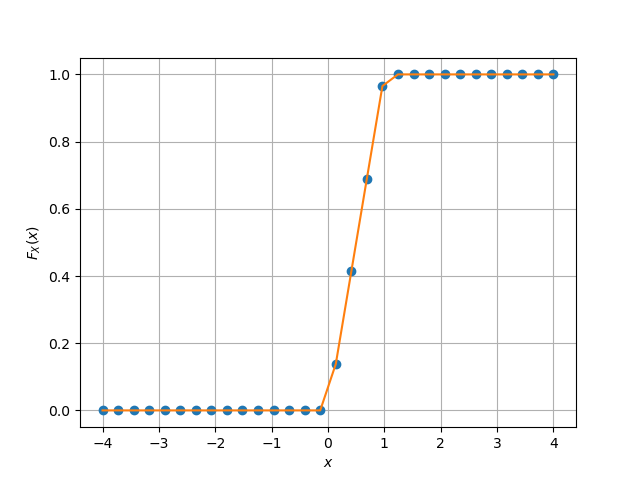
\includegraphics[width=\columnwidth]{./codes/1/fig/uni_cdf.png}
\caption{The CDF of $U$}
\label{fig:uni_cdf}
\end{figure}
%
\item
Find a  theoretical expression for $F_{U}(x)$.
\\ 
\solution $U$ is a Uniform Random Variable Distribution.\\
the PDF of the the distribution can be given as:

\begin{align}
		p_{U}(x) = 
		\begin{cases}
			1 & x \in [0, 1] \\
			0 & \text{otherwise}
		\end{cases}
\end{align}
\\
The CDF of $U$ is given by
	\begin{align}
		F_{U}(x) = \pr{U \le x} = \int_{-\infty}^x p_{U}(x) ~\mathrm{d}x
	\end{align}
	\\
Therefore, we obtain the CDF of $U$ as
	\begin{align}
		F_{U}(x) = 
		\begin{cases}
			0 & x < 0 \\
			x & 0 \le x \le 1 \\
			1 & x > 1
		\end{cases}
	\end{align}\\
	
\item
The mean of $U$ is defined as
%
\begin{equation}
E\sbrak{U} = \frac{1}{N}\sum_{i=1}^{N}U_i
\end{equation}
%
and its variance as
%
\begin{equation}
\text{var}\sbrak{U} = E\sbrak{U- E\sbrak{U}}^2 
\end{equation}

Write a C program to  find the mean and variance of $U$. \\
\solution Download the C source code by executing the following commands
\begin{lstlisting}
wget https://github.com/HARI-donk-EY/Rand_nums/blob/main/codes/1/mean_var_cal.c
wget https://github.com/HARI-donk-EY/Rand_nums/blob/main/codes/coeffs.h
\end{lstlisting}

Use the below command in the terminal to run code.
\begin{lstlisting}
gcc mean_var_cal.c -lm -o mean_var_cal.out
./mean_var_cal.out
\end{lstlisting}

From the code we get the output of the Mean as 0.500007, and Variance as 0.083301.\\

\item Verify your result theoretically given that
\end{enumerate}
%
\begin{equation}
E\sbrak{U^k} = \int_{-\infty}^{\infty}x^kdF_{U}(x)
\end{equation}\\

\solution We know that,
\begin{equation}
E\sbrak{U} = \int_{-\infty}^{\infty}xdF_{U}(x)
\end{equation}\\
On differentiation thr CDF obtained above, we get,
\begin{align}
		dF_{U}(x) = 
		\begin{cases}
			0 & x < 0 \\
			dx & 0 \le x \le 1 \\
			0 & x > 1
		\end{cases}
\end{align}
From this, we get,
\begin{equation}
	E\sbrak{U} = \int_{0}^{1}x dx = \frac{1}{2} = 0.5
\end{equation}\\
Similarly, 
\begin{align}
	E\sbrak{U^2} = \int_{0}^{1}x^2dx = \frac{1}{3}
\end{align}

From varience,
\begin{equation}
\text{var}\sbrak{U} = E\sbrak{U^2} - (E\sbrak{U})^2
\end{equation}\\
By substituting,
\begin{align}
	& = \frac{1}{3} - \brak{\frac{1}{2}}^2\\
	& = \frac{1}{12} \approx 0.083333
\end{align}\\

\section{Central Limit Theorem}
%
\begin{enumerate}[label=\thesection.\arabic*
,ref=\thesection.\theenumi]

%
\item
Generate $10^6$ samples of the random variable
%
\begin{equation}
X = \sum_{i=1}^{12}U_i -6
\end{equation}\\
%
using a C program, where $U_i, i = 1,2,\dots, 12$ are  a set of independent uniform random variables between 0 and 1
and save in a file called gau.dat\\
\solution Download the C source code by executing the following commands
\begin{lstlisting}
wget https://github.com/HARI-donk-EY/Rand_nums/blob/main/codes/2/gaugen.c
wget https://github.com/HARI-donk-EY/Rand_nums/blob/main/codes/coeffs.h

\end{lstlisting}
Compile and run the C program by executing the following
\begin{lstlisting}
gcc gaugen.c -lm -o gaugen.out
./gaugen.out
\end{lstlisting}
%
\item
Load gau.dat in python and plot the empirical CDF of $X$ using the samples in gau.dat. What properties does a CDF have?
\\
\solution  The following code plots Fig. \ref{fig:gauss_cdf}
\begin{lstlisting}
wget https://github.com/HARI-donk-EY/Rand_nums/blob/main/codes/2/cdf_plot_gau.py
\end{lstlisting}
Use the below command in the terminal to run code.
\begin{lstlisting}
python3 cdf_plot_gau.py
\end{lstlisting}

\begin{figure}
\centering
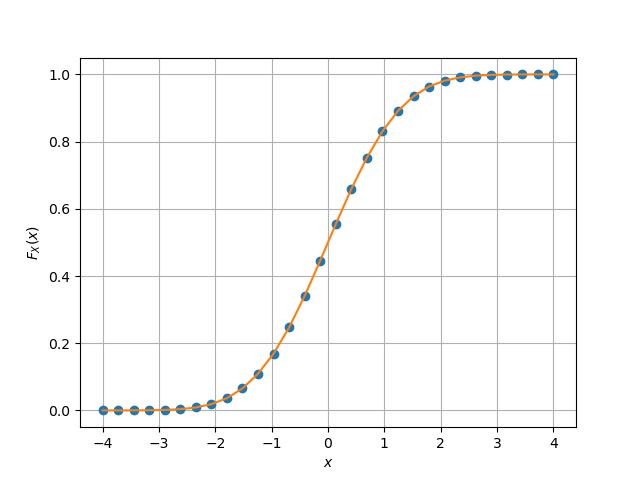
\includegraphics[width=\columnwidth]{./codes/2/fig/gauss_cdf.png}
\caption{The CDF of $X$}
\label{fig:gauss_cdf}
\end{figure}

Properties of this CDF are:
\begin{itemize}
	\item $F_{Z}(x)=P(Z \leq x)= 1-Q(x) $
    \item $\lim \limits_{x\rightarrow \infty} F_{Z}(x)=1, \hspace{5pt} \lim \limits_{x\rightarrow -\infty} F_{Z}(x)=0$
    \item  $F_{Z}(0)=\frac{1}{2}$
    \item  $F_{Z}(-x)=1-F_{Z}(x)$\\
\end{itemize}

\item
Load gau.dat in python and plot the empirical PDF of $X$ using the samples in gau.dat. The PDF of $X$ is defined as
\begin{align}
p_{X}(x) = \frac{d}{dx}F_{X}(x)
\end{align}
What properties does the PDF have?
\\
\solution Download the following Python code that plots Fig. \ref{fig:gauss_pdf}
\begin{lstlisting}
wget https://github.com/HARI-donk-EY/Rand_nums/blob/main/codes/2/pdf_plot.py
\end{lstlisting}
Run the code by executing
\begin{lstlisting}
python pdf_plot.py
\end{lstlisting}

The PDF graph is symmetric about $x=0$ and bell shaped. The mean of the graph is situated at the apex of the bell.\\

\begin{figure}
\centering
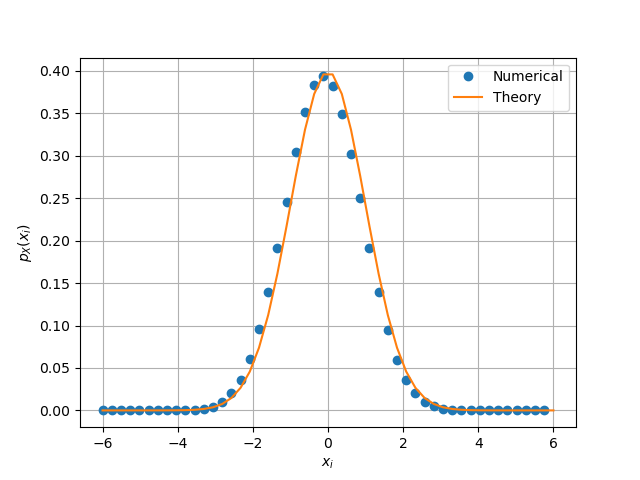
\includegraphics[width=\columnwidth]{./codes/2/fig/gauss_pdf.png}
\caption{The PDF of $X$}
\label{fig:gauss_pdf}
\end{figure}

\item Find the mean and variance of $X$ by writing a C program.\\

\solution Download the C source code by executing the following commands\\	
\begin{lstlisting}
wget https://github.com/HARI-donk-EY/Rand_nums/blob/main/codes/2/mean_var_cal.c
wget https://github.com/HARI-donk-EY/Rand_nums/blob/main/codes/coeffs.h
\end{lstlisting}

Use the below command in the terminal to run code.
\begin{lstlisting}
gcc mean_var_cal.c -lm -o mean_var_cal.out
./mean_var_cal.out
\end{lstlisting}

From the code we get the output of the Mean as 0.000294, and Variance as 0.999560.\\

\item Given that 
\begin{align}
p_{X}(x) = \frac{1}{\sqrt{2\pi}}\exp\brak{-\frac{x^2}{2}}, -\infty < x < \infty,
\end{align}
repeat the above exercise theoretically.\\
\solution From above, the Mean will be given as,
\begin{align}
	E\sbrak{X} & = \int_{-\infty}^{\infty} x p_{X}(x) dx \\
	& = \int_{-\infty}^{\infty} \frac{x}{\sqrt{2\pi}}\exp\brak{-\frac{x^2}{2}} dx \\
	& = \frac{1}{\sqrt{2\pi}}\int_{-\infty}^{\infty} x e^{-\frac{x^2}{2}} dx
\end{align}
\begin{align*}
	x e^{-\frac{x^2}{2}} \text{ is an odd function.}\\
	\text{Hence, }E\sbrak{X} = 0\\
\end{align*}
Similarly,
\begin{align}
E\sbrak{X^2} & = \int_{-\infty}^{\infty} x^2 p_{X}(x) dx \\
& = \int_{-\infty}^{\infty} \frac{x^2}{\sqrt{2\pi}}\exp\brak{-\frac{x^2}{2}} dx \\
& = 2 \int_{0}^{\infty} \frac{x^2}{\sqrt{2\pi}}\exp\brak{-\frac{x^2}{2}} dx \\
& = \sqrt{\frac{2}{\pi}} \int_{0}^{\infty} x \brak{x. \exp\brak{-\frac{x^2}{2}}} dx \\
\end{align}

Using integration by parts, we get,

\begin{multline}
= \sqrt{\frac{2}{\pi}} \brak{\left. x \int x \exp\brak{-\frac{x^2}{2}} dx}\right|_0^{\infty} \\- \sqrt{\frac{2}{\pi}}  \int_{0}^{\infty} 1 \cdot \int x \exp\brak{-\frac{x^2}{2}} dx\\
\end{multline}

\begin{align*}
& = \sqrt{\frac{2}{\pi}}\brak{\sbrak{-x\exp{-\frac{x^2}{2}}}_0^{\infty} - \int_0^{\infty}- \exp{\brak{-\frac{x^2}{2}}}}\\
& \text{Substituting } x \text{ with } t\sqrt{2},\\
& \text{And } dx \text{ with } dt\sqrt{2}\\
& = \sqrt{\frac{2}{\pi}}\brak{0 \  - \brak{-{\sqrt{2}} \int_0^{\infty} \exp(-t^2) \ dt}}\\
& = \sqrt{\frac{2}{\pi}}\brak{\sqrt{2} \int_0^{\infty} \exp(-t^2) \ dt}\\
& = \sqrt{\frac{2}{\pi}}\brak{\sqrt{2}\brak{\frac{\sqrt{\pi}}{2}}}\\
& = 1
\end{align*}
Therefore, Variance of $X$ will be,
\begin{align*}
var\brak{X} & = {E\sbrak{X}}^2 - E\sbrak{X^2}\\
& = 0-1 = 1\\
\end{align*}
\end{enumerate}

\newpage

\section{From Uniform to Other}
\begin{enumerate}[label=\thesection.\arabic*
,ref=\thesection.\theenumi]
%
\item
Generate samples of 
%
\begin{equation}
V = -2\ln\brak{1-U}
\end{equation}
%
and plot its CDF.  

\solution Download the C source code by executing the following commands
\begin{lstlisting}
wget https://github.com/HARI-donk-EY/Rand_nums/blob/main/codes/3/vgen.c
wget https://github.com/HARI-donk-EY/Rand_nums/blob/main/codes/coeffs.h

\end{lstlisting}
Compile and run the C program by executing the following
\begin{lstlisting}
gcc vgen.c -lm -o vgen.out
./vgen.out
\end{lstlisting}

The following code plots Fig. \ref{fig:vdat_cdf}
\begin{lstlisting}
wget https://github.com/HARI-donk-EY/Rand_nums/blob/main/codes/3/cdf_plot_vdat.py
\end{lstlisting}
Use the below command in the terminal to run code.
\begin{lstlisting}
python3 cdf_plot_vdat.py
\end{lstlisting}

\begin{figure}
\centering
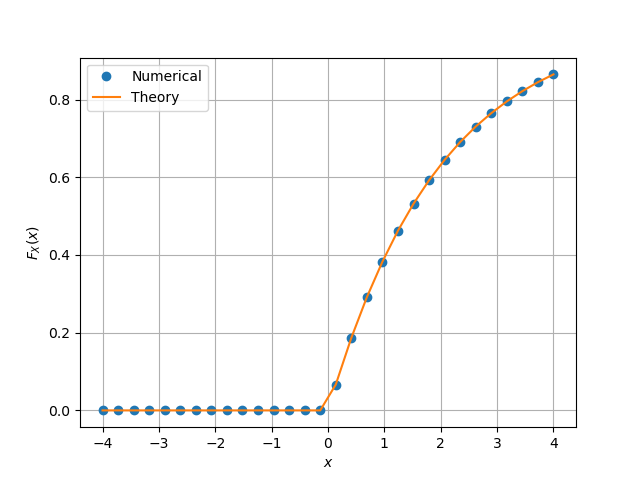
\includegraphics[width=\columnwidth]{./codes/3/fig/vdat_cdf.png}
\caption{The CDF of $V$}
\label{fig:vdat_cdf}
\end{figure}

\item Find a theoretical expression for $F_V(x)$.

\solution We have
\begin{align}
	F_V(x) &= \pr{V \le x} \\
	&= \pr{-2\ln\brak{1-U} \le x} \\
	&= \pr{\ln\brak{1-U} \ge -\frac{x}{2}} \\
	&= \pr{1-U \ge \exp\brak{-\frac{x}{2}}} \\
	&= \pr{U \le 1 - \exp\brak{-\frac{x}{2}}} \\
	&= F_U\brak{1 - \exp\brak{-\frac{x}{2}}}
\end{align}
Now,
\begin{align}
	0 \le 1-\exp\brak{-\frac{x}{2}} &< 1 \qquad \text{if } x \ge 0	\\	
	1-\exp\brak{-\frac{x}{2}} &< 0 \qquad \text{if } x < 0	
\end{align}

Therefore,
\begin{align}
	F_V(x) = 
	\begin{cases}
		1-\exp\brak{-\dfrac{x}{2}} & x \ge 0 \\
		0 & x < 0
	\end{cases}
\end{align}

\end{enumerate}

\section{Triangular Distribution}
\begin{enumerate}[label=\thesection.\arabic*
,ref=\thesection.\theenumi]
%
\item 
Generate
\begin{align*}
T & = U_1 + U_2\\
\end{align*}
\solution Download the C source code by executing the following commands
\begin{lstlisting}
wget https://github.com/HARI-donk-EY/Rand_nums/blob/main/codes/4/tritrien.c
wget https://github.com/HARI-donk-EY/Rand_nums/blob/main/codes/coeffs.h

\end{lstlisting}
Compile and run the C program by executing the following
\begin{lstlisting}
gcc trigen.c -lm -o trigen.out
./trigen.out
\end{lstlisting}

\item
Find the $CDF$ of $T$.\\
\solution The $CDF$ of $T$ is given by:
\begin{align}
F_T(t) = \pr{T \leq t} = \pr{U_1 + U_2 \leq t}
\end{align}

\end{enumerate}

\end{document}
